% This file was created with tikzplotlib v0.10.1.
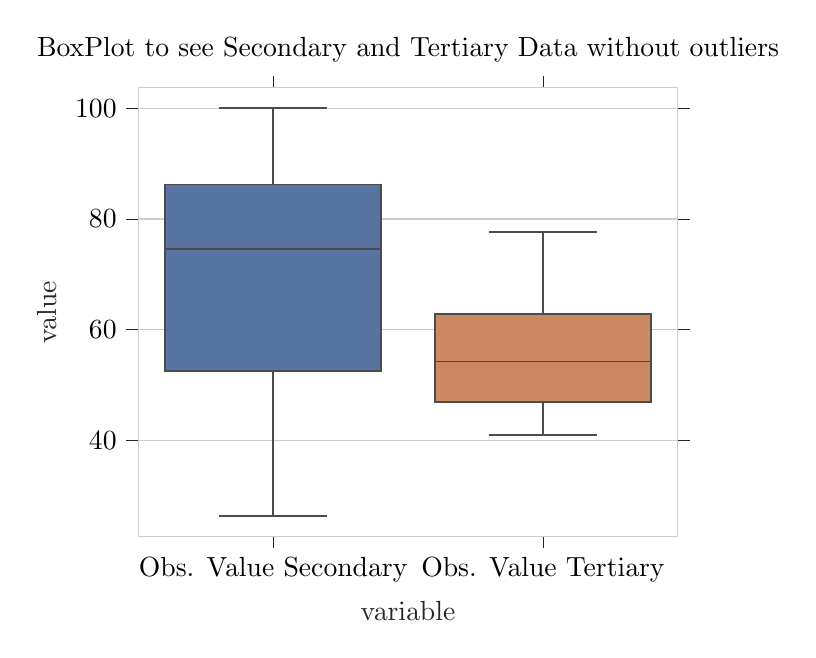
\begin{tikzpicture}

\definecolor{darkslategray38}{RGB}{38,38,38}
\definecolor{darkslategray76}{RGB}{76,76,76}
\definecolor{lightgray204}{RGB}{204,204,204}
\definecolor{peru20313699}{RGB}{203,136,99}
\definecolor{steelblue88116163}{RGB}{88,116,163}

\begin{axis}[
axis line style={lightgray204},
tick align=outside,
title={BoxPlot to see Secondary and Tertiary Data without outliers},
x grid style={lightgray204},
xlabel=\textcolor{darkslategray38}{variable},
xmajorticks=true,
xmin=-0.5, xmax=1.5,
xtick style={color=darkslategray38},
xtick={0,1},
xticklabels={Obs. Value Secondary,Obs. Value Tertiary},
y grid style={lightgray204},
ylabel=\textcolor{darkslategray38}{value},
ymajorgrids,
ymajorticks=true,
ymin=22.722793, ymax=103.679867,
ytick style={color=darkslategray38}
]
\path [draw=darkslategray76, fill=steelblue88116163, semithick]
(axis cs:-0.4,52.5594411333436)
--(axis cs:0.4,52.5594411333436)
--(axis cs:0.4,86.2092675)
--(axis cs:-0.4,86.2092675)
--(axis cs:-0.4,52.5594411333436)
--cycle;
\path [draw=darkslategray76, fill=peru20313699, semithick]
(axis cs:0.6,47.01373)
--(axis cs:1.4,47.01373)
--(axis cs:1.4,62.82417)
--(axis cs:0.6,62.82417)
--(axis cs:0.6,47.01373)
--cycle;
\addplot [semithick, darkslategray76]
table {%
0 52.5594411333436
0 26.40266
};
\addplot [semithick, darkslategray76]
table {%
0 86.2092675
0 100
};
\addplot [semithick, darkslategray76]
table {%
-0.2 26.40266
0.2 26.40266
};
\addplot [semithick, darkslategray76]
table {%
-0.2 100
0.2 100
};
\addplot [semithick, darkslategray76]
table {%
1 47.01373
1 40.98805
};
\addplot [semithick, darkslategray76]
table {%
1 62.82417
1 77.64571
};
\addplot [semithick, darkslategray76]
table {%
0.8 40.98805
1.2 40.98805
};
\addplot [semithick, darkslategray76]
table {%
0.8 77.64571
1.2 77.64571
};
\addplot [semithick, darkslategray76]
table {%
-0.4 74.57505
0.4 74.57505
};
\addplot [semithick, darkslategray76]
table {%
0.6 54.24357
1.4 54.24357
};
\end{axis}

\end{tikzpicture}
